\documentclass[xcolor={dvipsnames},pdf, hyperref={colorlinks=true, citecolor=ForestGreen, linkcolor=BlueViolet, urlcolor=Magenta}]{beamer}
\usetheme{Frankfurt}  
\usecolortheme{whale}
\usepackage{tikz} 
\usepackage{graphicx}
\usepackage{dsfont}
\usepackage{hyperref}
\usepackage{alltt}
\usepackage{enumerate}
\usepackage{amsthm}
\theoremstyle{definition}
\newtheorem{exmp}{Example}[section]
\usepackage{verbatim}               % useful for \begin{comment} and \end{comment}
\usepackage{eurosym}                % used for euro symbol
\usepackage{caption} 
\usepackage{graphicx}
\usepackage{adjustbox}
\graphicspath{{Figures/}}
\usepackage{subcaption}
\usepackage{color}
\usepackage{float}
\usepackage{amssymb}
\usepackage{sgamevar}
\usepackage{remreset}% tiny package containing just the \@removefromreset command
\makeatletter
\@removefromreset{subsection}{section}
\makeatother
\setcounter{subsection}{1}


\newcommand{\defn}[1]{\textbf{#1}}


%Instructor version
\newcommand{\blank}[0]{}
\newcommand{\ddp}[1]{{\textcolor{ForestGreen}{#1}}} 
\newcommand{\dd}[1]{{\underline{\textcolor{ForestGreen}{#1}}}}

%Student version
%\newcommand{\blank}[0]{\vspace{2em}}
%\newcommand{\dd}[1]{\underline{\hspace{3cm}}} 
%\newcommand{\ddp}[1]{}

\addtobeamertemplate{navigation symbols}{}{%
	\usebeamerfont{footline}%
	\usebeamercolor[fg]{footline}%
	\hspace{1em}%
	\insertframenumber/\inserttotalframenumber
}

\section{Economic Growth}

%% preamble
\title{Economic Growth}
\author{David A. D\'iaz}
\institute{UNC Chapel Hill}
\date{}

\AtBeginSection[] %Section links on slides

\begin{document} 
	
	\begin{frame}
		
		\titlepage
		
	\end{frame}


\begin{frame}{Economic Growth}
\begin{itemize}
	\item \textbf{Principle 8: A Country's Standard of Living Depends on Its Ability to Produce Goods and Services}
	\item There is obviously much variation in the standard of living across the world, and even within countries. This section explores the long-run determinants of real GDP and its growth over time.
\end{itemize}
\end{frame}

\begin{frame}{Motivation}
\begin{figure}
	\centering
	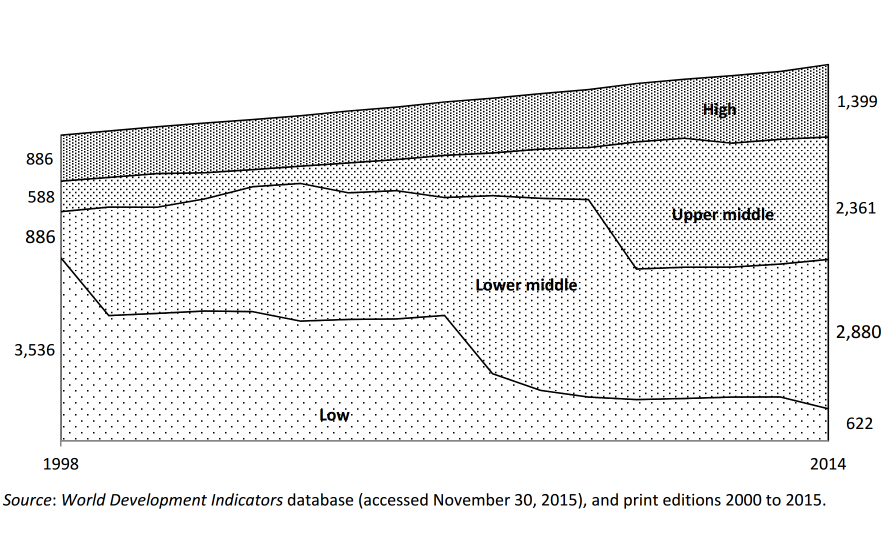
\includegraphics[scale=.90]{04D_1}
\end{figure}
\end{frame}

\begin{frame}{Motivation}
	\begin{figure}
		\centering
		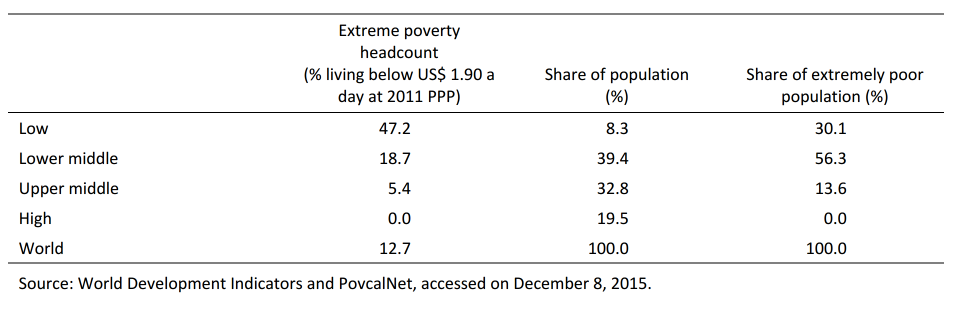
\includegraphics[scale=.90]{04D_2}
	\end{figure}
\end{frame}

\begin{frame}{Motivation}
	\begin{figure}
		\centering
		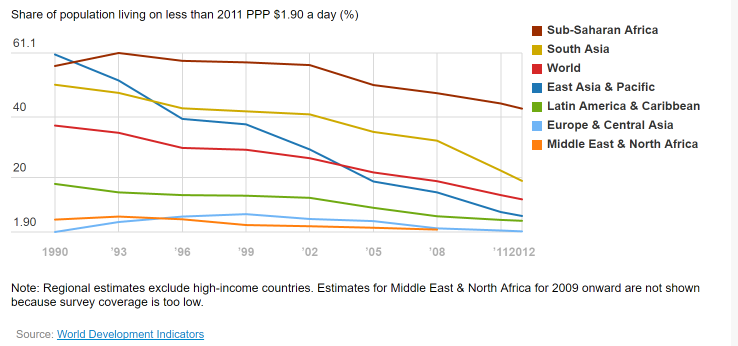
\includegraphics[scale=1.25]{04D_3}
	\end{figure}
\end{frame}


\begin{frame}{Economic Growth}
\begin{exmp} 
	
	Suppose the United States currently has a real GDP per capita of \$30,000 and it grows 3\% every year. Additionally, China has a real GDP per capita of \$15,000, but its growth rate is 7\%. What will be real GDP per capita in each country in 10 years? In 20 years?
\end{exmp}
\ddp{\pause US: \\
	GDP$_{2015}$ = 30K\\
	\pause GDP$_{2025}$ = 30K(1.03)$^{10}$ = 40,317\\
	\pause GDP$_{2035}$ = 30K(1.03)$^{20}$ = 54,183\\ 
	China: \\ 
	GDP$_{2015}$ = 15K\\
	\pause GDP$_{2025}$ = 15K(1.07)$^{10}$ = 29,507\\
	\pause GDP$_{2035}$ = 15K(1.07)$^{20}$ = 58,045}
\end{frame}

\begin{frame}{Economic Growth}
\begin{itemize}
	\item \defn{The Rule of 70:} An approximation for how long it takes a variable growing at a constant rate to double. 
	\[T_2 \approx 70/g\]
	where g is in \% terms.
\end{itemize}
\end{frame}

\section{How Nations Grow}

\begin{frame}{Economic Growth}
\begin{exmp}
	How many years will it take the US to double their per capita GDP if their real GDP per capita continues to grow at 3\% each year? China?
\end{exmp}
\ddp{\pause US: 70/3 $\approx$ 23.33 years \\
	\pause China: 70/7 $\approx$ 10 years}
\end{frame}

\begin{frame}{Economic Growth}
\begin{itemize}
	\item \defn{Productivity:} The quantity of goods and services produced from each unit of labor input.
	\item The determinants of productivity:
	\begin{enumerate}
		\item \defn{Physical capital:} The stock of equipment and structures that are used to produced goods and services.
		\item \defn{Human capital:} The knowledge and skills that workers acquire through education, training, and experience.
		\item \defn{Natural resources:} The inputs into the production of goods and services that are provided by nature.
		\item \defn{Technological knowledge:} Society's understanding of the best ways to produce goods and services. Includes common knowledge, trade secretes, and patents.
	\end{enumerate}
\end{itemize}
\end{frame}

\begin{frame}{The Role of Government}
\begin{itemize}
	\item \defn{Institutions:} The ``Rules of the game'' that shape interactions and structure economic incentives. 
	\item Includes formal laws/regulations and social norms. 
	\item They are the \underline{ultimate} causes of growth.
	\item Institutions can encourage economic prosperity through (i) establishing property rights, (ii) an honest government, (iii) political stability, (iv) a dependable legal system, and (v) competitive and open markets.
\end{itemize}
\end{frame}

\begin{frame}{The Role of Government}
\begin{itemize}
	\item \textbf{Saving and Investment}: Investing more in capital goods today will lead to more capital goods tomorrow and increase in goods and services in the future. Trade-off is that consumption today must decrease.
	\item \textbf{Investment from abroad}: Investments increase the stock of capital and lead to increases in productivity and wages.
\end{itemize}
\end{frame}


\begin{frame}{The Role of Government}
\begin{itemize}
	\item \textbf{Education}: Investment in human capital leads to increases in productivity. Additionally, there are spillovers or positive externalities from education and training
	\item \textbf{Health and nutrition}: Investment in human capital. Healthier individuals are more productive.
\end{itemize}
\end{frame}

\begin{frame}{The Role of Government}
\begin{itemize}
	\item \textbf{Property rights and political stability}: Property rights - The ability of people to exercise authority over the resources they own. Threats to property rights: lack of enforcement, corruption, fraud, and political instability. Lack of property rights discourages investment and prevents markets from operating efficiently.
\end{itemize}
\end{frame}

\begin{frame}{The Role of Government}
\begin{itemize}
	\item \textbf{Free trade}: Gains from trade increase economic prosperity. Trade restrictions (e.g., tariffs, quotas) decrease prosperity. Geography plays a role here (e.g., access to trade)
	\item \textbf{Research and Development}: Technological advances by private research and the government increase productivity. Incentives such as grants, patents can motivate individuals/companies to innovate.
\end{itemize}
\end{frame}

\begin{frame}{The Role of Government}
\begin{itemize}

\item \textbf{Population growth}: Large populations have more workers to produce goods, but also more people to consume goods/services (counter-acting). More over, capital is diluted. Malthus: stretch of natural resources is outweighed by gains in productivity growth. Larger population might promote greater technological growth.
\end{itemize}
\end{frame}

\begin{frame}{Readings and Assignments}
\begin{itemize}
	\item Today: Mankiw Ch. 25
	\item Next time: Solow Model videos
	\item Problem Set 5, section 1
\end{itemize}
\end{frame}

\end{document}